\chapter{Klasifikasi Teks}

\section{Klasifikasi Teks}
Merupakan suatu cara dalam memilah milah data teks berdasarkan pada parameter dengan data yang bersifat dokumen ataupun teks yang memiliki kumpulan teks didalamnya, Untuk tipe data teks sendiri yaitu bertipe data char dan string yang mudah untuk diolah

\section{Klasifikasi bunga tidak dapat menggunakan machine learning}
Karena memiliki masalah input yang sama namun keluarannya berbeda (output), jika terjadi error pada inputan maka disebut dengan ‘noise’. Noise sendiri merupakan suatu output yang disimpan/ditangkap maupun direkap bukan seperti seharusnya (keluaran yang diinginkan).

\section{Teknik pembelajaran mesin pada teks pada kata-kata yang digunakan di youtube }
Pada saat menggunakan Youtube terdapat Machine Learning yang bekerja dan memproses perintah
ataupun aktivitas tersebut, dimana akan memfilter secara otomatis video yang disesuaikan
dengan "keyword" yang kita masukkan sehingga memberikan keluaran video dengan keyword yang benar. Adapula fitur yang didapatkan ketika sedang menonton youtube. Pada tampilan sebelah kanan terdapat pilihan 'Next' ataupun 'Suggestion' yang menampilkan video serupa sesuai dengan kita cari atau sedang di tonton.

\section{Vektorisasi Data}
Vektorisasi data adalah proses normalisasi data teks dengan pemberian nilai terhadap setiap fitur. Pada penelitian ini digunakan teknik TF-IDF untuk pemberian bobot fitur. Teknik ini akan menghitung nilai Term Frequency (TF) dan Inverse Document Frequency (IDF) pada setiap fitur di setiap dokumen dalam korpus

\section{Bag-of-words}
Bag-of-words merupakan suatu representasi penyederhanaan yang digunakan dalam suatu pemrosesan Bahasa alami dan dapat mengambil informasi. Model bag-of-words sederhana untuk dipahami dan diterapkan dan juga dapat diandalkan dalam menangani masalah pemodelan Bahasa dan klasifikasi dokumen. Pada model ini, tiap kalimat dalam dokumen digambarkan sebagai token

\section{TFIDF}
tf–idf, TF*IDF, atau TFIDF adalah ukuran statistik yang menggambarkan pentingnya suatu istilah terhadap sebuah dokumen dalam sebuah kumpulan atau korpus. Ukuran ini sering dipakai sebagai faktor pembobot dalam pencarian temu balik informasi, penambangan teks, dan pemodelan pengguna.


\section{Praktikum}
\subsection{Aplikasi Sederhana Menggunakan Pandas}
\begin{figure}[!htbp]
	\centering

	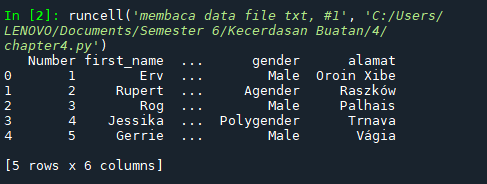
\includegraphics[width=10cm,height=4cm]{figures/Cp4-1.png}
	\caption{Aplikasi sederhana menggunakan pandas}
	\label{penanda}
\end{figure}
\textbf{Penjelasan Code Aplikasi Sederhana pandas perbaris :}
\begin{itemize}
	\item Langkah awal yaitu di line Pertama merupakan langkah mengimport library pandas kemudian di inisialisasi menjadi pd
	\item Untuk bagian Variable data di definisikan data data untuk kolom nama, kolom npm dan kolom angkatan
	\item Lalu membuat variabel dengan nama data dan mengisinya dengan data dummy yang sudah dibuat
	\item Selanjutnya dilihat 5 baris pertama dan banyaknya baris data
\end{itemize}

\subsection{Praktek dataframe tersebut dipecah menjadi dua dataframe yaitu 450 row pertama dan 50 row sisanya}
\begin{figure}[!htbp]
	\centering
	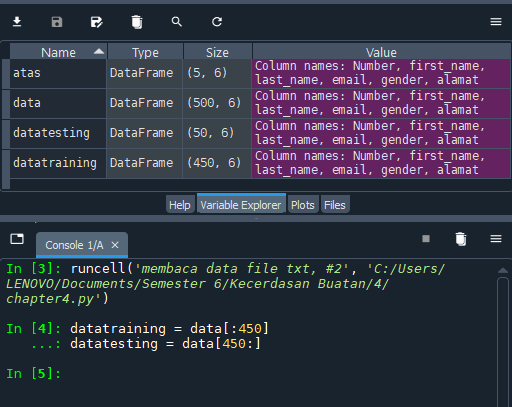
\includegraphics[width=10cm,height=2cm]{figures/Cp4-2.png}
	\caption{Vektorisasi dan Klasifikasi data}
	\label{penanda}
\end{figure}
\textbf{Penjelasan Code hasil pemecahan data perbaris :}
\begin{itemize}
	\item Membuat 2 buah data frame yang pertama 450 data dan yang kedua 50 data
	\item data tersebut terdapat data training dan data testing
\end{itemize}

\subsection{vektorisasi dan klasifikasi dari data (NPM mod 4, jika 0 maka katty
	perry, 1 LMFAO, 2 Eminem, 3 Shakira) dengan Decission Tree}
\begin{figure}[!htbp]
	\centering
	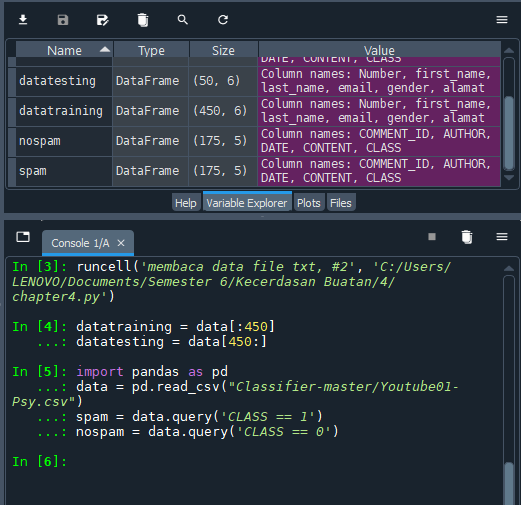
\includegraphics[width=6cm,height=6cm]{figures/Cp4-3.png}
	\caption{Vektorisasi dan Klasifikasi data}
	\label{penanda}
\end{figure}
\textbf{Penjelasan Code Aplikasi Sederhana numpy perbaris :}
\begin{itemize}
	\item Baris Pertama Yaitu import library pandas kemudian di inisialisasi menjadi pd
	\item Melakukan fungsi bag of word dengan cara menghitung semua kata
	\item Melakukan bag of word pada dataframe pada colom CONTENT
	\item Melihat isi vektorisasi
	\item Menampilkan isi data pada baris ke 300
	\item Mengambil apa saja nama kolom yang tersedia
	\item Melakukan randomisasi agar hasil sempurna pada klasifikasi
	\item Membuat data training dan testing
	\item melakukan training pada data training dan di vektorisasi
	\item melakukan testing pada data testing dan di vektorisasi
	\item Dimana akan mengambil label span dan bukan spam
\end{itemize}

\subsection{klasifikasikan dari data vektorisasi dengan klasifikasi SVM}
\begin{figure}[!htbp]
	\centering
	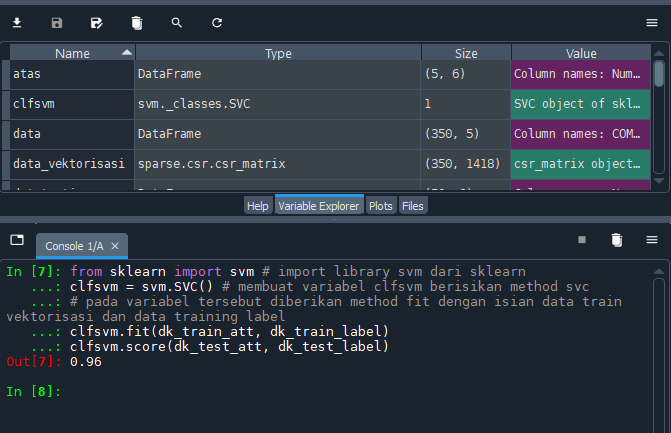
\includegraphics[width=6cm,height=6cm]{figures/Cp4-4.png}
	\caption{Vektorisasi dan Klasifikasi data dengan klasifikasi SVM}
	\label{penanda}
\end{figure}
\textbf{Penjelasan Code klasifikasikan dari data vektorisasi dengan klasifikasi SVM perbaris :}
\begin{itemize}
	\item Baris Pertama Yaitu import library svm dari sklear
	\item membuat variabel clfsvm berisikan method svc
	\item pada variabel tersebut diberikan method fit dengan isian data train vektorisasi dan data training label
\end{itemize}

\subsection{klasifikasikan dari data vektorisasi dengan klasifikasi Decission Tree}
\begin{figure}[!htbp]
	\centering
	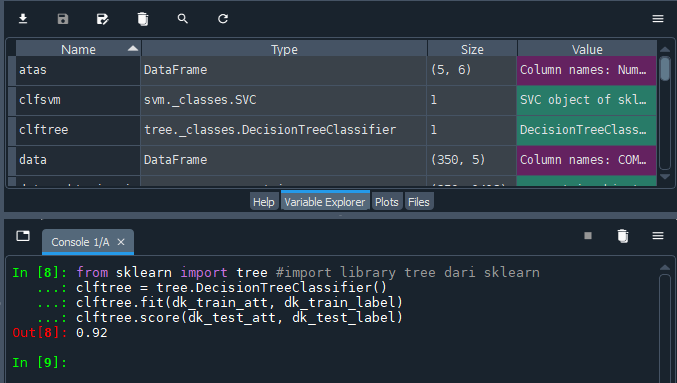
\includegraphics[width=6cm,height=6cm]{figures/Cp4-5.png}
	\caption{Vektorisasi dan Klasifikasi data dengan klasifikasi Decission Tree}
	\label{penanda}
\end{figure}
\textbf{Penjelasan Code klasifikasikan dari data vektorisasi dengan klasifikasi Decission Tree perbaris :}
\begin{itemize}
	\item Baris Pertama Yaitu import library tree dari sklearn
\end{itemize}

\subsection{Plot confusion matrix menggunakan matplotlib}
\begin{figure}[!htbp]
	\centering
	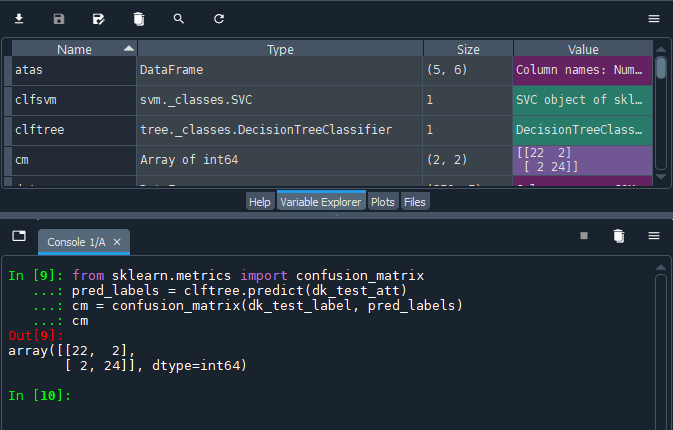
\includegraphics[width=6cm,height=6cm]{figures/Cp4-6.png}
	\caption{Plot confusion matrix menggunakan matplotlib}
	\label{penanda}
\end{figure}
\textbf{Penjelasan Code Plot confusion matrix menggunakan matplotlib perbaris :}
\begin{itemize}
	\item Baris Pertama Yaitu import library confusion matrix dari sklearn metrics
	\item lalu dipanggil lagi cm yaitu confusion matrix yang didalamnya ada dktest label dan pred labels
\end{itemize}

\subsection{Program Cross Validation}
\begin{figure}[!htbp]
	\centering
	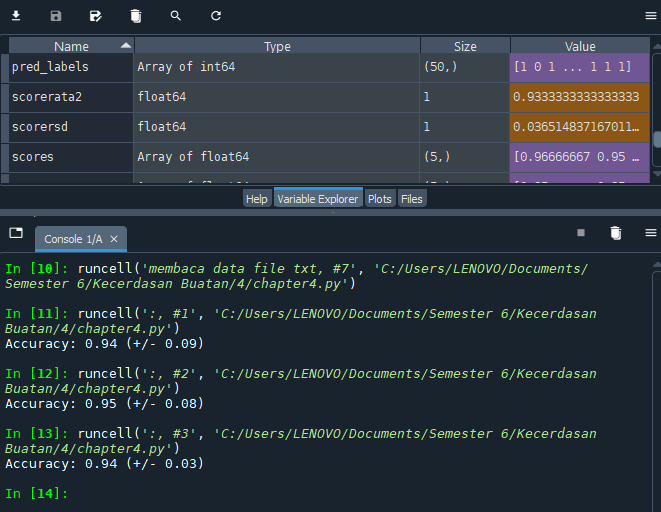
\includegraphics[width=6cm,height=6cm]{figures/Cp4-7.png}
	\caption{Program Cross Validation}
	\label{penanda}
\end{figure}
\textbf{Penjelasan Program Cross Validation perbaris :}
\begin{itemize}
	\item Baris Pertama Yaitu import library cross val score dari sklearn model selection
	\item Lalu menampilkan hasil dari scores
	\item Selanjutnya menampilkan hasil dari scores tree
	\item Dan terakhir itu menampilkan hasil dari scoressvm
\end{itemize}

\subsection{Program Pengamatan Komponen Informasi}
\begin{figure}[!htbp]
	\centering
	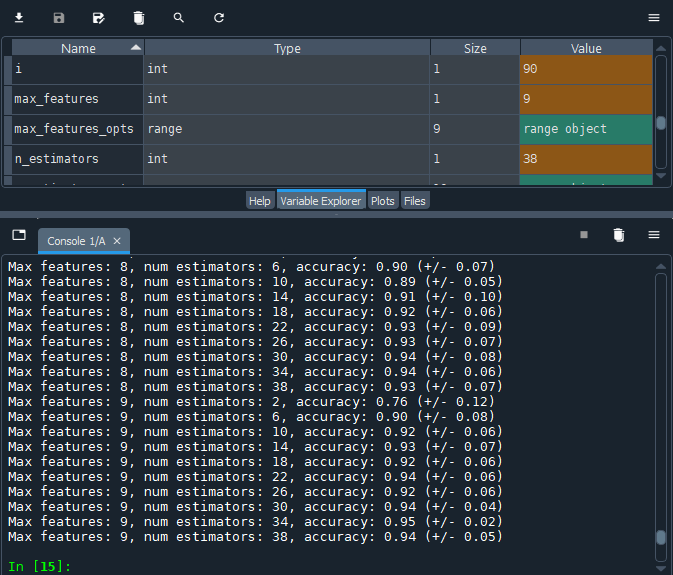
\includegraphics[width=6cm,height=6cm]{figures/Cp4-8.png}
	\caption{Program Pengamatan Komponen Informasi}
	\label{penanda}
\end{figure}
\textbf{Penjelasan Program Pengamatan Komponen Informasi perbaris :}
\begin{itemize}
	\item Baris Pertama Yaitu import numpy yang diinisialisasikan menjadi np
	\item import library RandomForestClassifier dari sklearn ensemble
\end{itemize}

\subsection{Gambar Hasil Akhir}
\begin{figure}[!htbp]
	\centering
	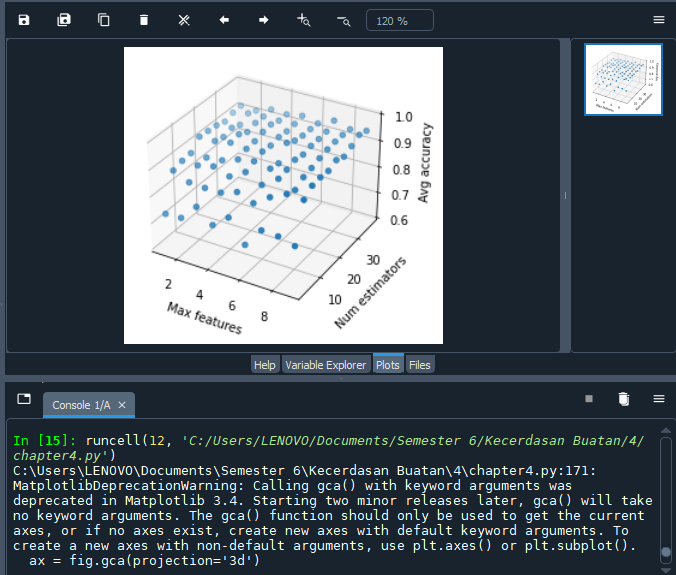
\includegraphics[width=6cm,height=6cm]{figures/Cp4-9.png}
	\caption{Gambar Hasil akhir chapter 4}
	\label{penanda}
\end{figure}
\textbf{Penjelasan Gambar Hasil akhir chapter 4 perbaris :}
\begin{itemize}
	\item Baris Pertama Yaitu import matplotlib pyplot yang diinisialisasikan menjadi plt
	\item import library Axes3D dari mpl toolkits mplot3d
	\item import cm dari matplotlib
	\item lalu disesuaikan ukuran dan juga letak (posisi) untuk gambarnya nanti. 
	\item Selanjutnya atur bagian posisi xyz
	\item lalu show (menampilkan gambar)
\end{itemize}
